\label{fs-framework}

Our task is to design a framework for end-to-end text streams multi-classification that overcomes the challenges mentioned above. We assume that there are two types of input streams: pre-labeled and raw. The latter stream elements must be labeled by a classifier and delivered to end-user. The pre-labeled stream is used for updating a machine learning model with new data.

\begin{figure}[htbp]
  \centering
  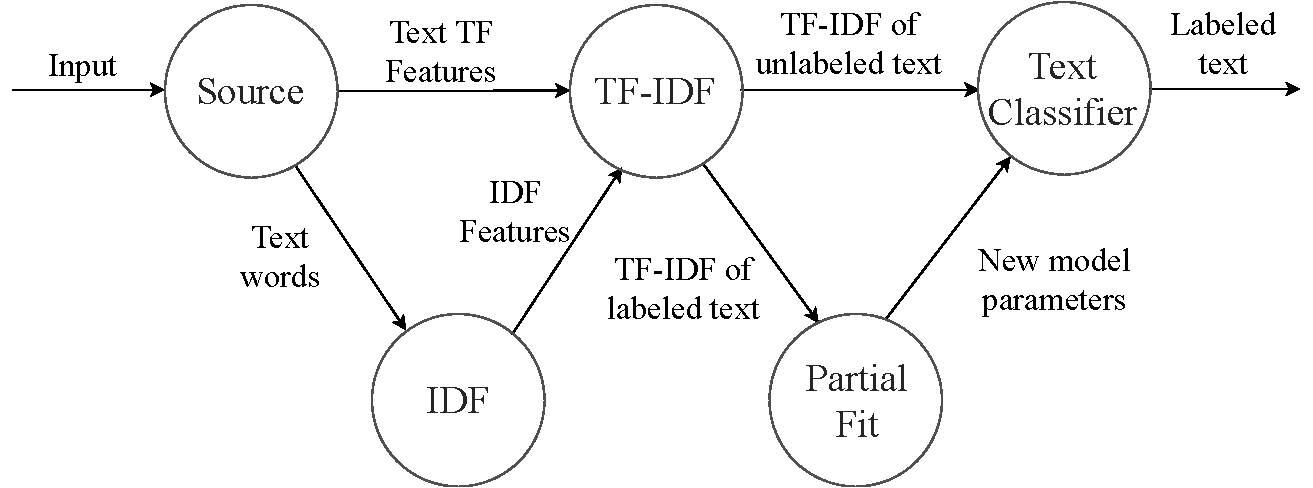
\includegraphics[scale=0.48]{pics/logical-graph}
  \caption{The logical graph}
  \label {logical_graph}
\end{figure}

\subsection{Data flow \label{DF}}

\subsubsection{Predicting pipeline}

Typical text pipeline consists of the following steps. The first one is processing by Bag-of-words model. For these vectors, computing TF-IDF features is applied, where TF is a term frequency, and IDF is an inverse document frequency. The last one is training a classifier on these features. In order to adapt this pipeline of this pipeline for stream processing engine, there is a need to represent it in the form of so-called {\em logical graph}. It serves as a descriptive language for defining streaming computations. Vertices of a logical graph denote operations, while edges indicate data subscriptions between them. 

The initial point in our data flow is an {\em Input} vertex. It receives input texts from data producers and computes term frequencies right away. Computing of inverse document frequencies is a separate operation because it maintains a state and requires different data partitioning in a physical execution that we touch upon further. {\em TF-IDF} vertex joins features corresponding to the same text and passes them to the {\em Text Classifier}. {\em Text Classifier} is the very last vertex that predicts a label and delivers it to a data consumer. The scheme of the proposed logical graph is shown in Figure~\ref{logical_graph}.

\begin{figure}[htbp]
  \centering
  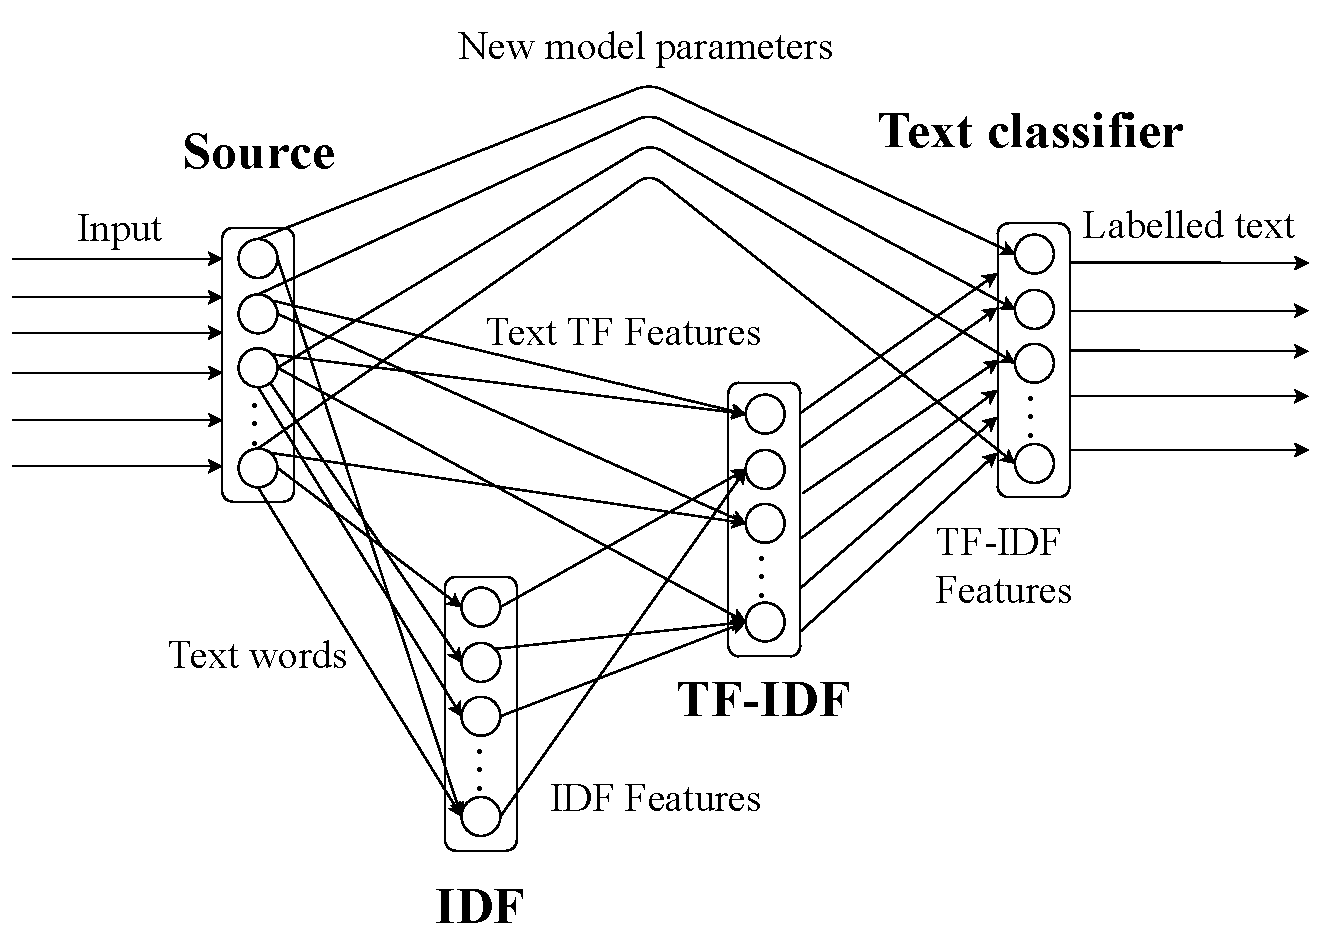
\includegraphics[scale=0.375]{pics/physical-graph}
  \caption{The physical graph}
  \label {physical_graph}
\end{figure}

Usually, in stream processing systems, all operations from a logical graph execute on all computational units. Scalability is achieved due to data partitioning before each operation. Figure ~\ref{physical_graph} captures the scheme of a physical execution for the proposed logical graph. Each vertex on the scheme denotes the same computational cluster consisted of multiple units. Data partitioning before {\em IDF} and {\em TF-IDF} operations is defined by keys. Data elements with the same keys process on a single computational unit. For {\em IDF} operation the key is a word, while {\em TF-IDF} aggregates items with the same text identifier. As we can see, all operations that take part in predicting pipeline scales among all computational units. 

\subsubsection{Training pipeline}

Training pipeline is a separate branch within the logical graph introduced above. For already labeled text its features are sent to a {\em Partial fit} vertex instead of the {\em Classifier}. {\em Partial fit} vertex buffers all input elements until training is triggered. It is done using a distinct input stream element, which is submitted directly to the {\em Input}. Every vertex except the {\em Partial fit} passes this element through without processing. This behavior is similar to punctuations handling~\cite{tucker2003exploiting}. After training, the buffer flushes. Updated parameters of a machine learning model are saved for further training and broadcasted to all {\em Text Classifier} vertices.

\subsubsection{Dealing with concept drift}

Concept drift refers to the particular meaning of words, which changes over time. This aspect may affect the quality of a prediction, especially for data from news and social media sources. To handle this trait, we compute inverse document frequencies within a sliding window. The length of a window must coincide with a period of the additional training. Similar approach demonstrates its effectiveness in~\cite{klinkenberg2000detecting}.

\subsubsection{Stream processing engines}

The execution of the physical graph in the mentioned stream systems contains difficulties. The two data partitions may produce the non-deterministic results, which means no guarantee that independent runs on the same data will produce the same results. Also, due to the described above reasons, our pipeline requires exactly-once processing. 

In the Table~\ref{comparison} state-of-the-art stream systems are presented. As we can see, most of the systems demonstrate a lack of the needed properties or high latency for having them. FlameStream and MillWheel are two exceptions, however, the latter is a proprietary project, which cannot be used by anyone. Hence, our computations based on \FlameStream\, which provides both determinism and exactly once guarantee under low latency requirements. The mechanisms behind these features are detailed in~\cite{we2018adbis, we2018beyondmr}.

\begin{table}[htbp]

\begin{threeparttable}
\begin{tabular}{lccl}

System             & Determinism & Exactly-once & Latency    \\
\hline
FlameStream        &      +     &    +    &   low            \\
MillWheel          &      +     &    +    &   NA             \\
Spark Streaming    &      +     &    +    &   high           \\
Flink              &      --     &    +    &   high$^*$       \\
Storm              &      --     &    --    &   low            \\

\end{tabular}

* with enabled exactly-once

\end{threeparttable}

\caption{Stream processing systems comparison}
\label{comparison}
\end{table}

\subsection{Machine learning model \label{ML}}

In order to be efficiently embedded in the proposed data flow, several properties of machine learning model are desirable. A model should support the prior parameters and be able to train fast enough for real-time processing. The fast performance also includes a small size of the model for storing and updating operations in reasonable time and space.

The model can be chosen independently from other computations. In our case, we use Multinomial Logistic Regression. The training consists of the following formula:

\begin{center}

$$ J(W) = -\frac{1}{m} \sum \limits_{i = 1}^{m} \sum \limits_{j = 1}^{k} \mathbbm{1}_{\left\{y^{(i)} == j\right\}} \cdot \log \frac{\exp\left({W_{j}^Tx^{(i)}}\right) }{\sum \limits_{l = 1}^{k}  \exp\left({W_{l}^Tx^{(i)}}\right) }$$ 
 $$ +  \lambda_1 ||W||_1 + \lambda_2 ||W - W_{prev}||_2 $$

\end{center} 

The number of points in a new dataset is denoted as $m$. The point with index $i$ is shown as $x^{(i)}$. The number of classes is $k$. New weights are designated as $W$. The weights that computed in the previous step are $W_{prev}$. At the first time of triggering the process, $W_{prev}$ can be provided by a pre-train process.  

The formula provides the goal of the training. The first component is the standard softmax function for multiple classes. The second component keeps the l1 regularization of the weights, and provides sparsity, hence, the model has a small size -- about 1 Mb, which can be stored and updated with low cost. To use the previous history of the classifier weights, we apply l2 regularization as the third component. 

We are interested in finding such $W$ that minimizes $J(W)$. Taking derivatives, one can show that the gradient for each class component is:

\begin{center}

$$ \nabla_{W_j} \; J(W) = -\frac{1}{m} \sum \limits_{i = 1}^{m} \left[ x^{(i)} \left( \mathbbm{1}_{\left\{y^{(i)} == j\right\} } - \frac{\exp\left({W_{j}^Tx^{(i)}}\right)}{\sum \limits_{l = 1}^{k}  \exp\left({W_{l}^Tx^{(i)}}\right)} \right) \right] $$
$$ - \; \lambda_1 sign\left(W\right) - \frac{\lambda_2}{2} \left(W - W_{prev} \right), \; j = [1..k] $$

\end{center} 

We use Stochastic Gradient Descent for optimization. In experiments ~\ref{fs-short-experiments} section, model performance is presented.